\chapter{Конструкторская часть}
В данном разделе будет рассмотрены схемы исследуемого алгоритма.

\section{Схемы алгоритмов}

На рисунке 2.1 представлена схема однопоточного алгоритма блочной сортировки.

На рисунке 2.2 представлена схема алгоритма сортировки вставками, используемой для сортировки каждого блока.

На рисунке 2.3 представлена схема распараллеленного алгоритма блочной сортировки.

\begin{figure}[h!]
	\centering
	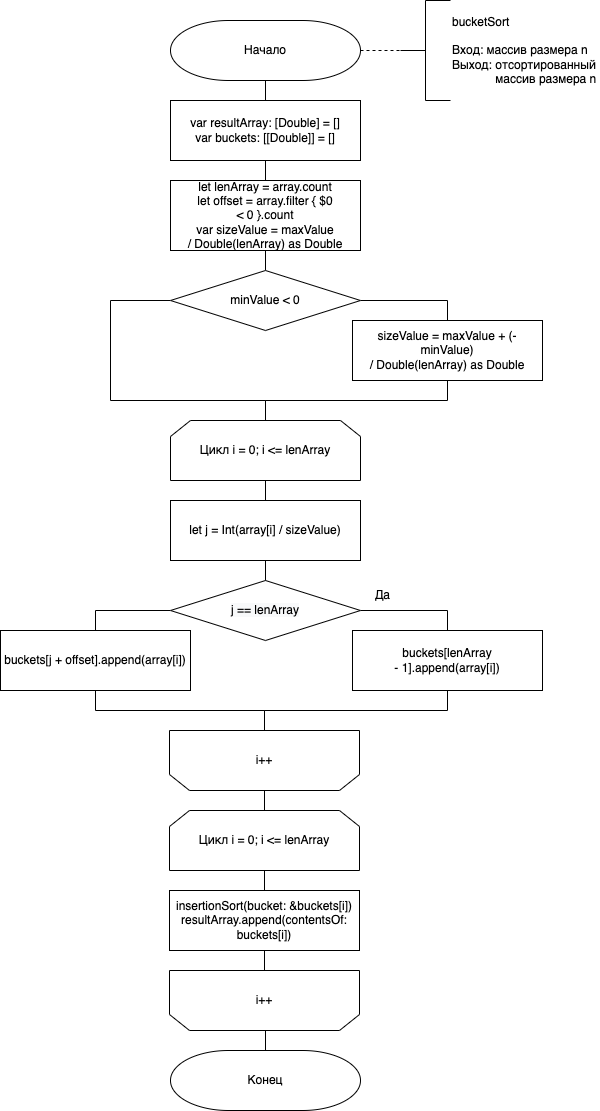
\includegraphics[width=0.8\linewidth]{img/Bucket.png}
	\caption{Схема алгоритма блочной сортировки}
	\label{fig:mpr}
\end{figure}

\begin{figure}[h!]
	\centering
	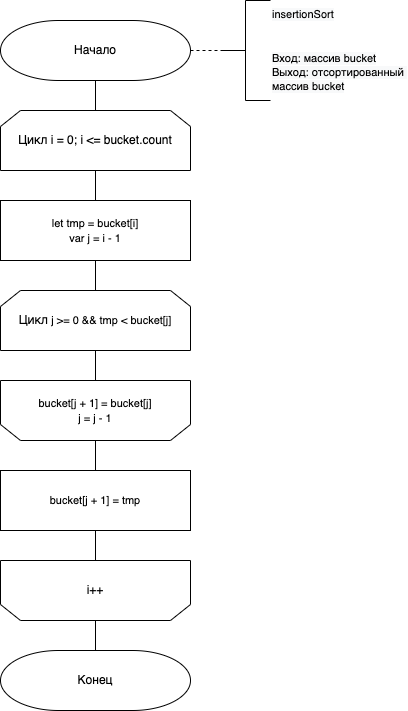
\includegraphics[width=0.8\linewidth]{img/Insertion.png}
	\caption{Схема алгоритма блочной сортировки}
	\label{fig:mpr}
\end{figure}

\begin{figure}[h!]
	\centering
	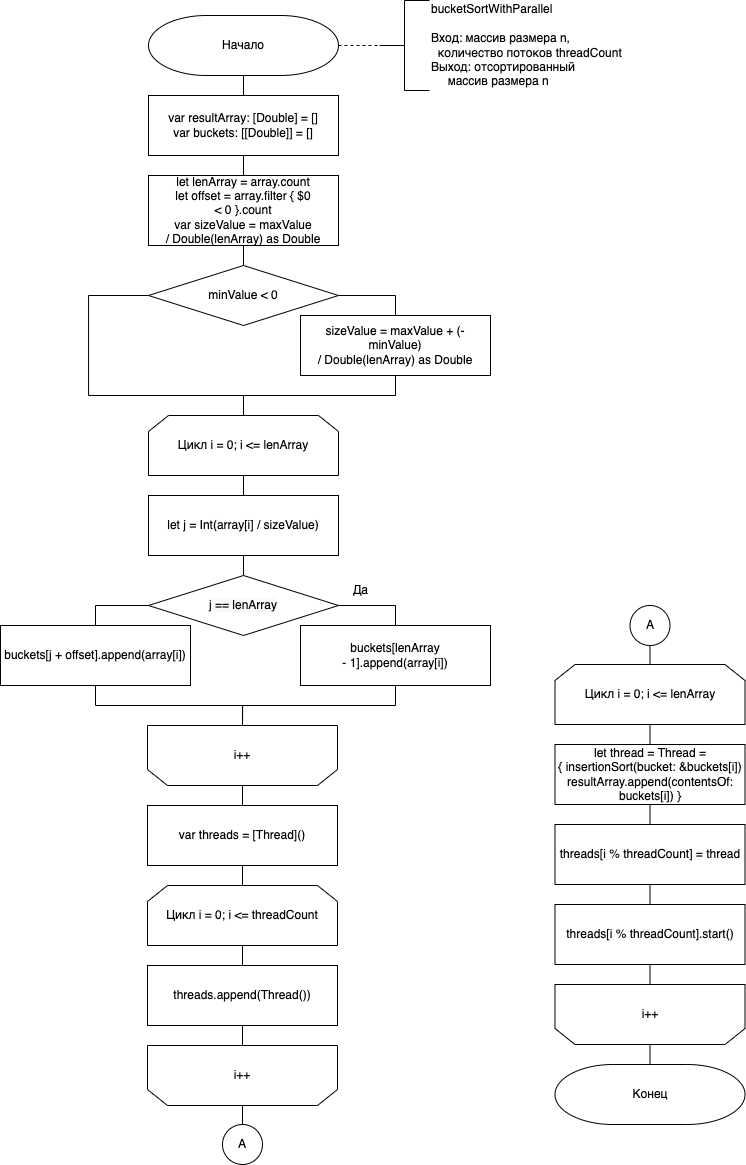
\includegraphics[width=0.95\linewidth]{img/BucketParallel.png}
	\caption{Схема алгоритма блочной сортировки}
	\label{fig:mpr}
\end{figure}


\section{Вывод}
На основе теоретических данных, полученных из аналитического раздела, была построена схема стандартного алгоритма блочной сортировки, а также, после разделения алгоритма на этапы, была предложена схема параллельного выполнения этапов.
